The results from analyses with this data will be displayed in three plots,
generated automatically during processing. 

\subsubsection{Score plot}
Figure \ref{fig:all} displays the raw results as a point plot per algorithm and
dataset.

\subsubsection{Ordering plot}
The ranking plot is intended to be a quick way of ordering algorithms, based on
the statistical significance returned by the procedure described in Section
\ref{stats}. Greyed-out squares show situations in which the y-axis pipeline did
not significantly improve over the x-axis pipeline; values in green squares show
the standardized mean difference over all datasets for that particular
pair. 

\subsubsection{Paired plot}
Figures \ref{fig:am} and \ref{fig:csp} show ranking plots. In order to look at
two algorithms in more detail, for particular pairs of algorithms we also offer
a plot of the score in one versus the score in the other, for all subjects
across all datasets. This is computed for all pairs of algorithms, and we show a
selection here that details results for some of the better-known methods.

\subsubsection{Time plot}
Figure \ref{fig:time} shows a plot of accuracy versus fitting time for the
model. In addition to accuracy, model fitting time can also affect which
pipeline is most appropriate for a given situation, though obviously
poor-performing models are not ideal regardless of accuracy. As there is a large
variety in channels and trial numbers among the datasets in this analysis, we
can infer the sensitivity of the fitting to the input size from the variance in
the X direction, and the range of scores from the Y direction. The best pipeline
would lie in the top right, while the worst would be in the bottom left.

Figure \ref{fig:all} shows all the results generated by this entire processing
chain. Surprisingly, perhaps, the pipelines do not clearly cluster on the
dataset level, making it unclear which ones perform best from simply this
plot. What is very clear, however, is that different datasets have very
different average scores independent of pipeline. The overall ranking of
algortihms can be found in Figure \ref{fig:rank}.

Figure \ref{fig:am} shows the pairwise comparison of the log
variance-based pipeline with CSP and the tangent space SVM. What is
very clearly shown both in the plots and the statistics is that, for
within-session scoring, it is strongly out-performed by both.

Figure \ref{fig:csp} shows the pairwise comparison of 
plain CSP with the two regularized approaches and with
tangent space SVM. For both the regularized approaches. while there is
a great deal of variance across subjects, the score from CSP and the
regularized CSP roughly track each other, such that there is no
significant difference between them. The only significant difference
is with the tangent space method.

Figure \ref{fig:time} shows how all the described methods compare in terms of
processing time. The methods based on Riemannian computation are more
computationally expensive at large sample sizes than the other methods (due to
the iterative computations and the increase in feature number).

\begin{figure*}
    \centering
    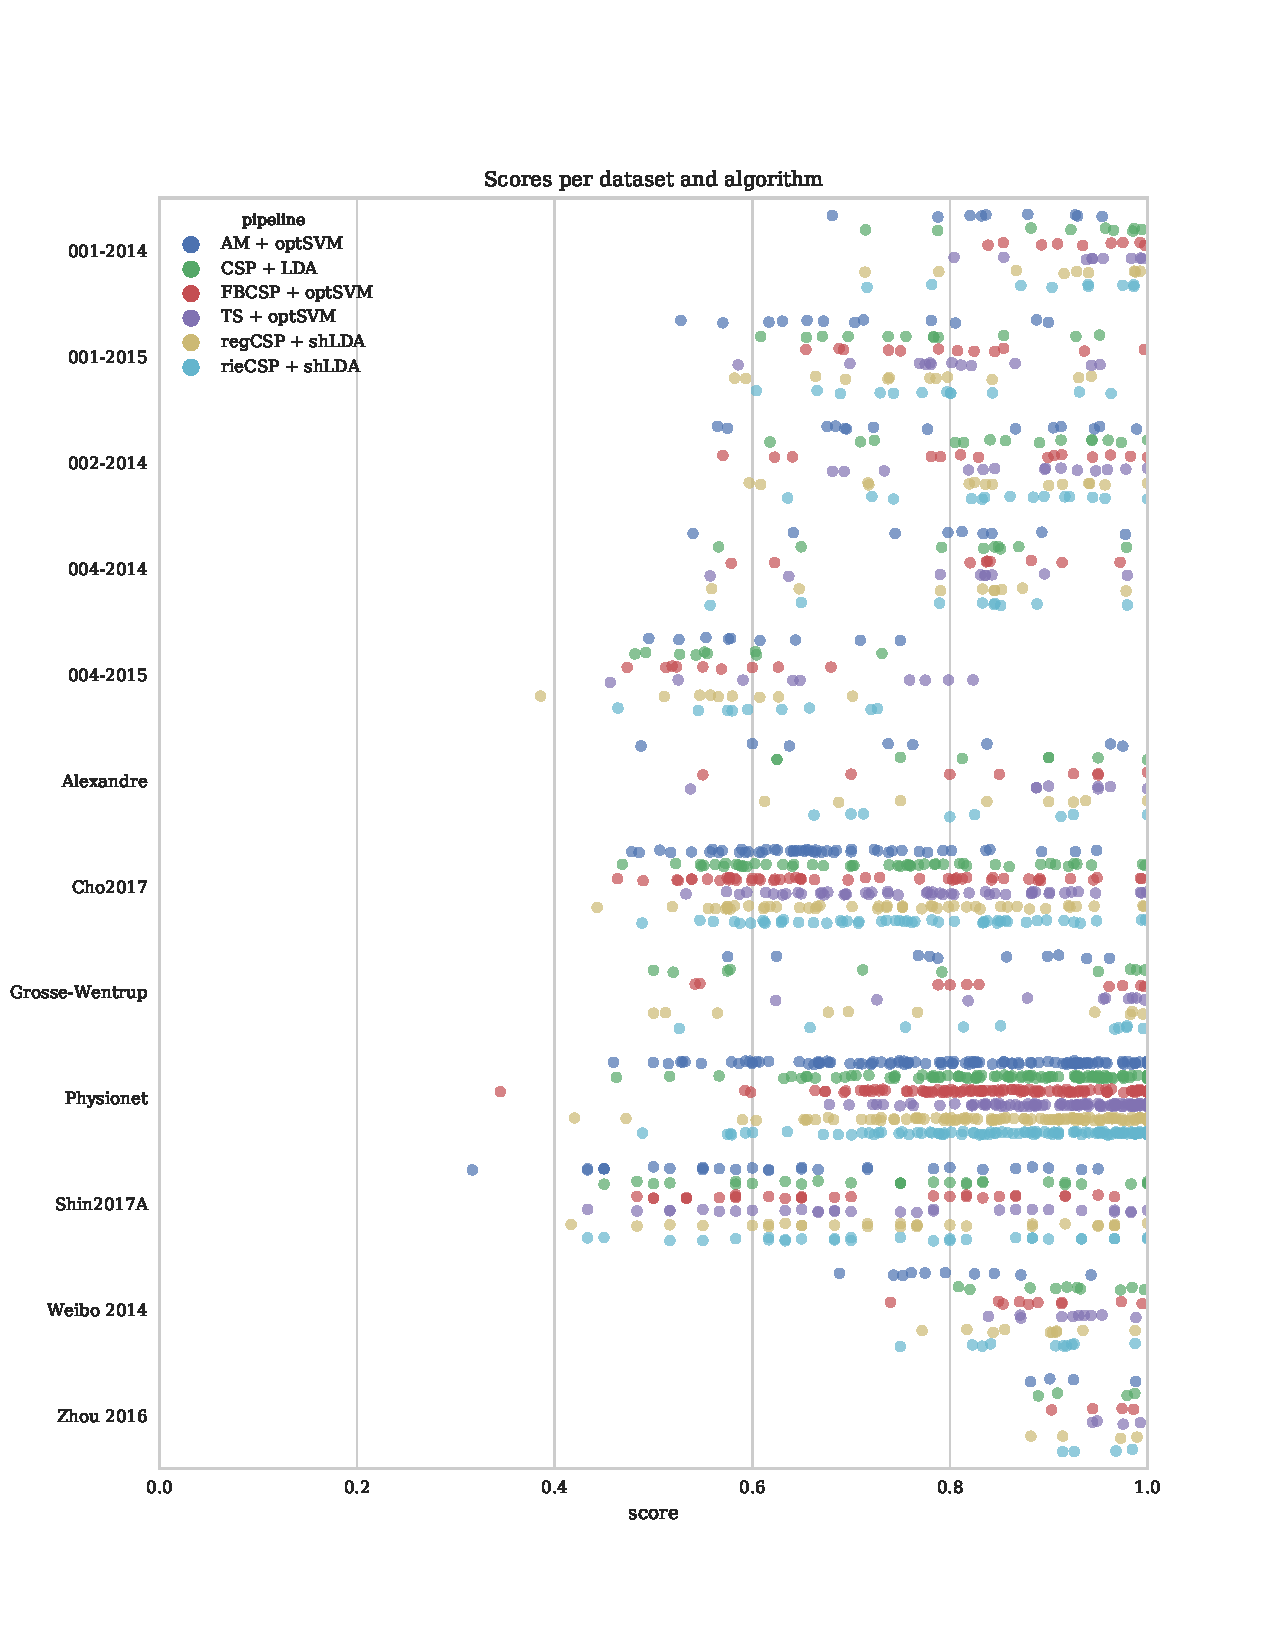
\includegraphics[width=\textwidth]{Figures/scores.pdf}
    \caption{Visualization of all generated scores, across all datasets.}
    \label{fig:all}
\end{figure*}


\begin{figure*}
    \centering
    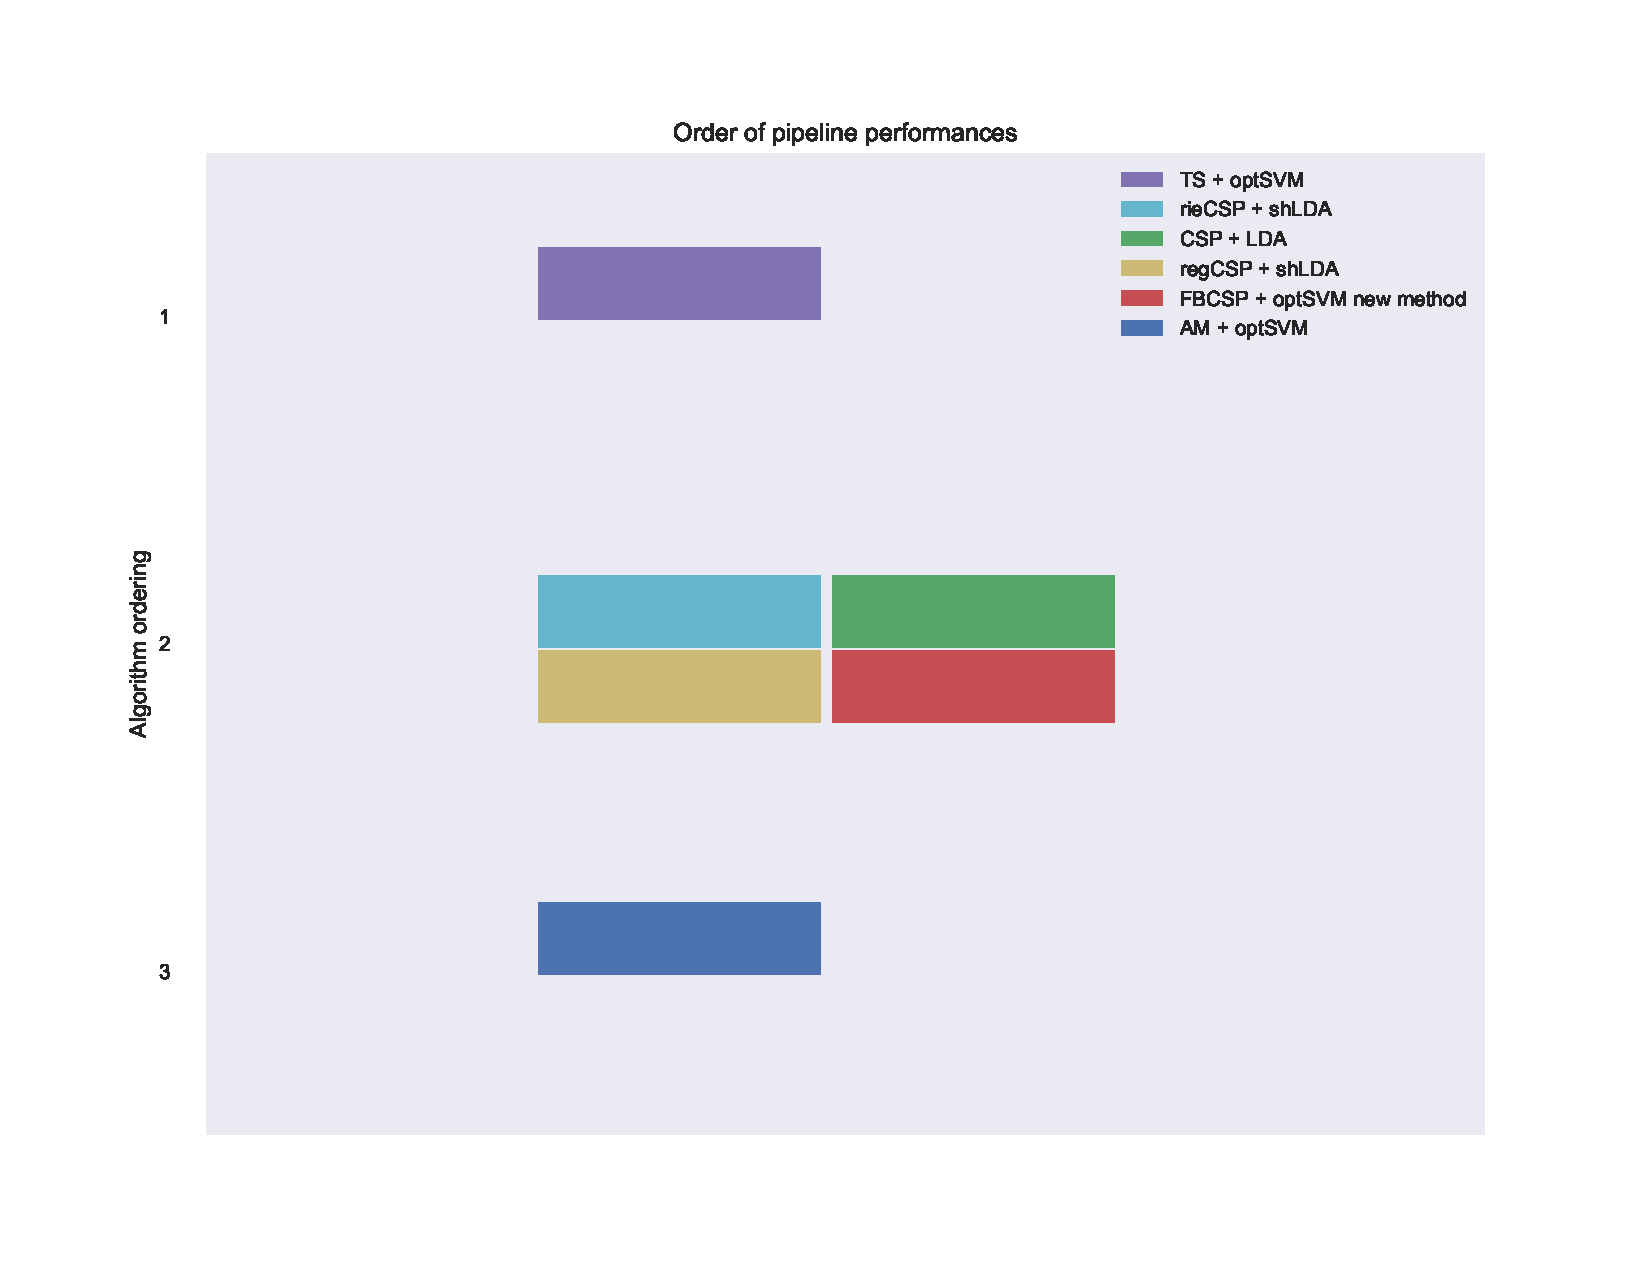
\includegraphics[width=\textwidth]{Figures/ordering.pdf}
    \caption{Ranking of algorithms in performance across all datasets with
      statistics generated as defined in section \ref{stats}. The numbers
      correspond to the standardized mean difference of the score in the y-axis
      minus that in the x-axis; grey boxes represent pairs where the algorithm
      on the y-axis is not significantly larger than the algorithm on the x. }
    \label{fig:rank}
\end{figure*}


\begin{figure*}
    \centering
    \begin{subfigure}{0.5\textwidth}
        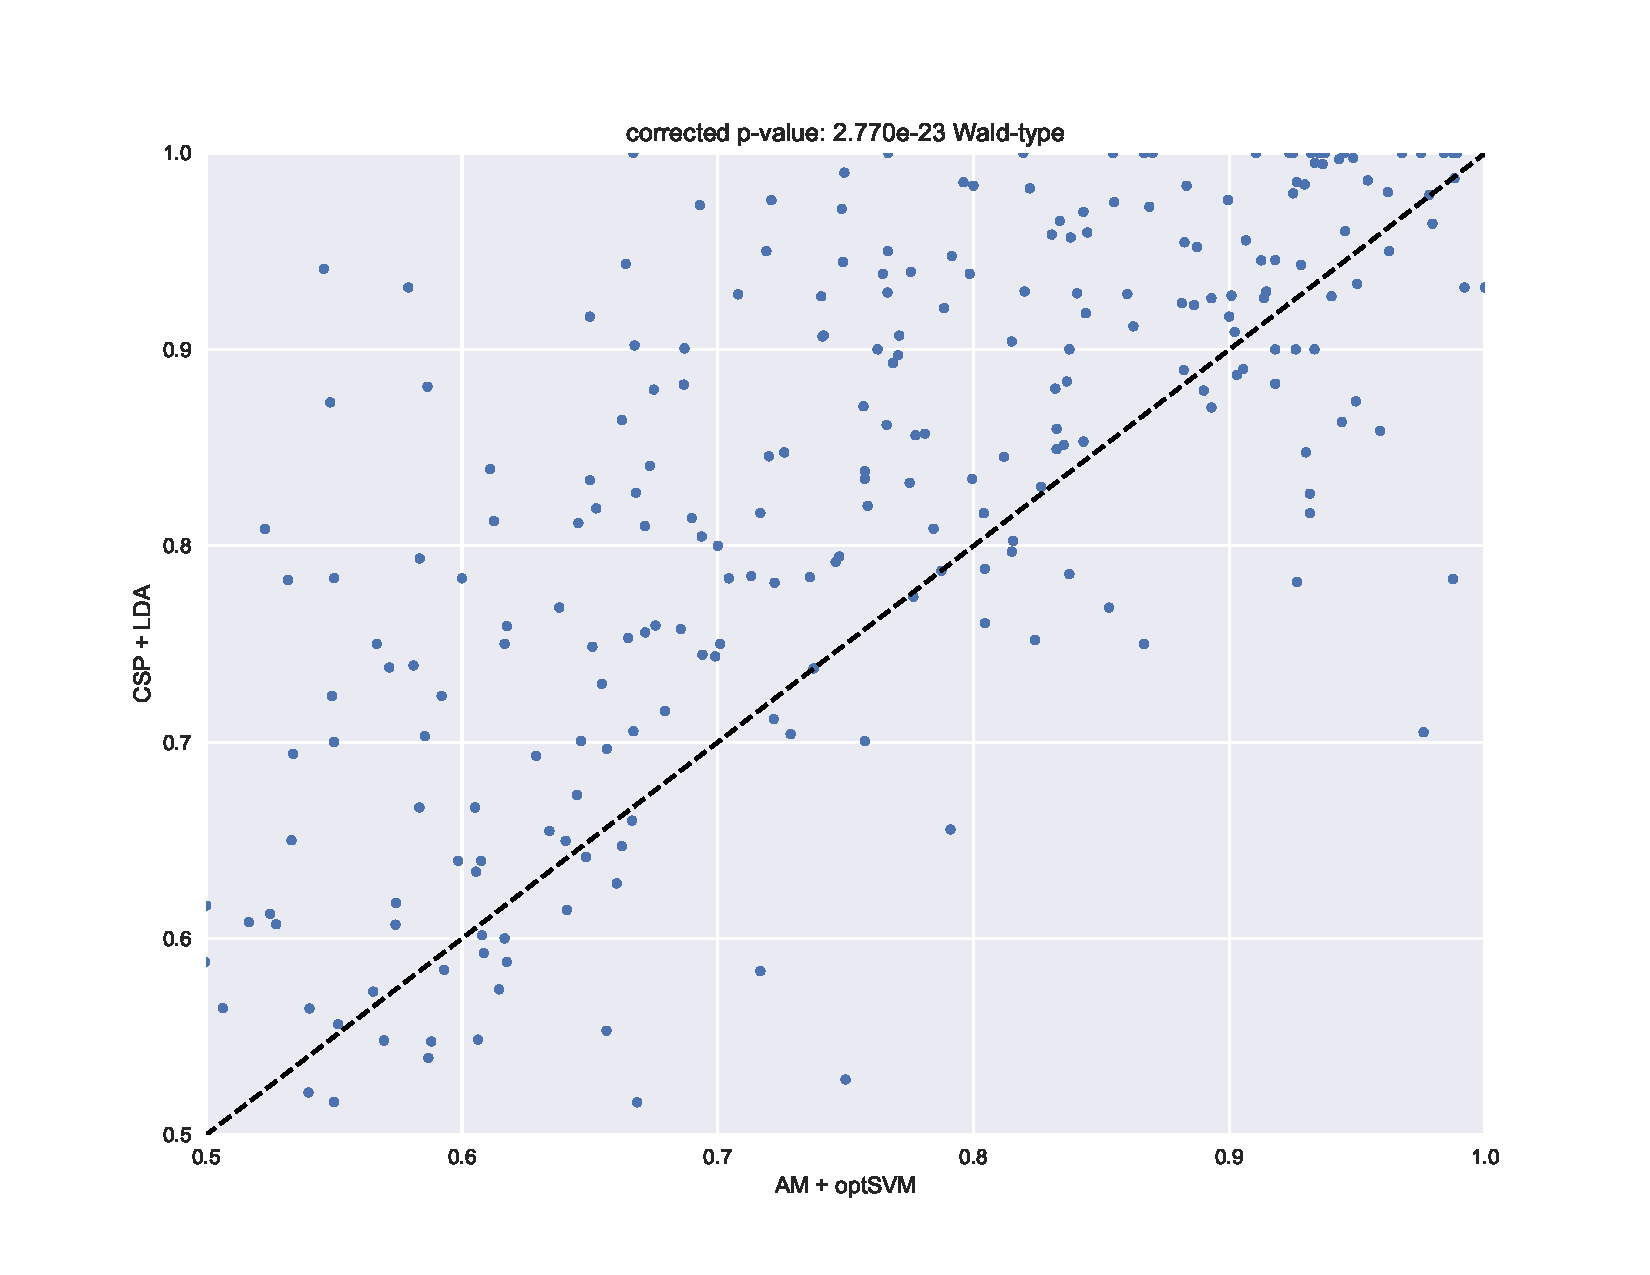
\includegraphics[width=\textwidth]{Figures/AM1.pdf}
    \end{subfigure}%
    \begin{subfigure}{0.5\textwidth}
        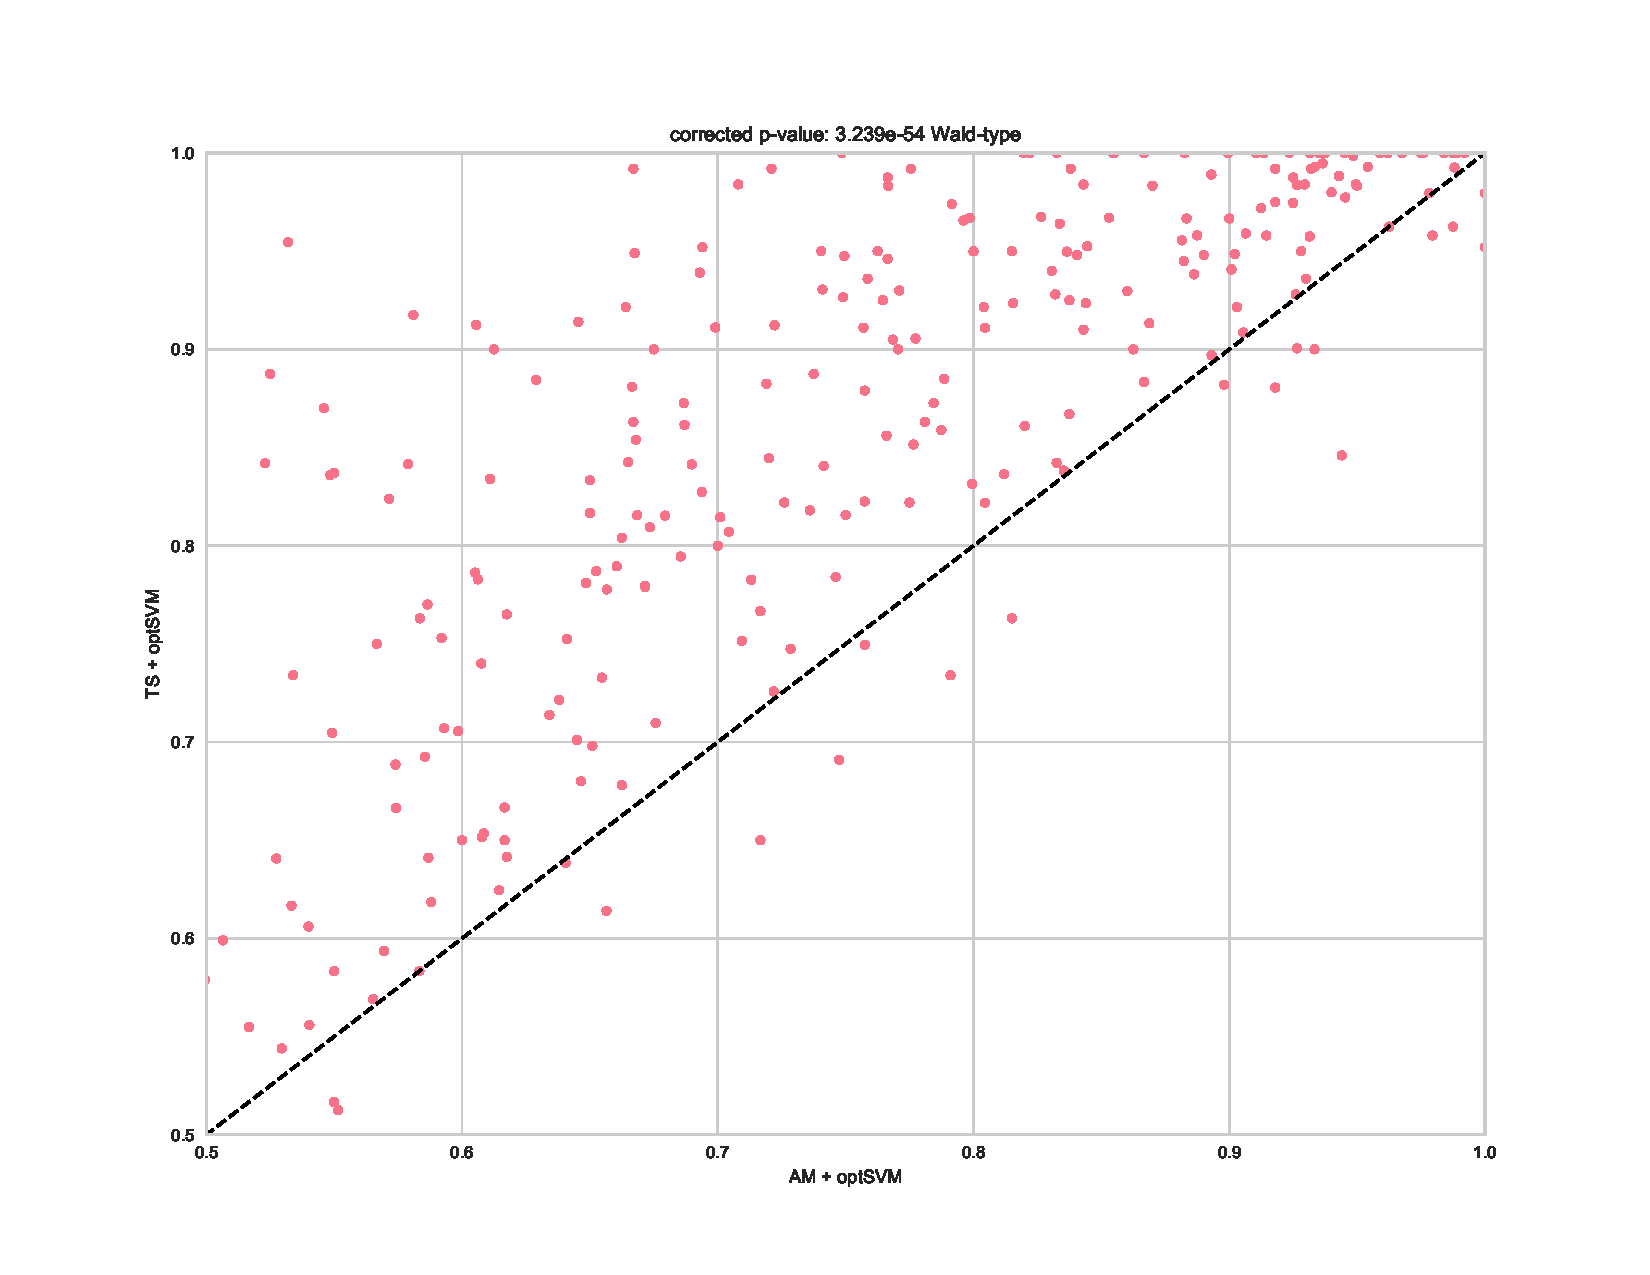
\includegraphics[width=\textwidth]{Figures/AM2.pdf}
    \end{subfigure}
    \caption{Paired plots of log variance versus basic CSP and the
      tangent space projection. It does
      consistently worse than both CSP and the tangent space method.}
    \label{fig:am}
\end{figure*}
\begin{figure*}
    \centering
    \begin{subfigure}{0.475\textwidth}
        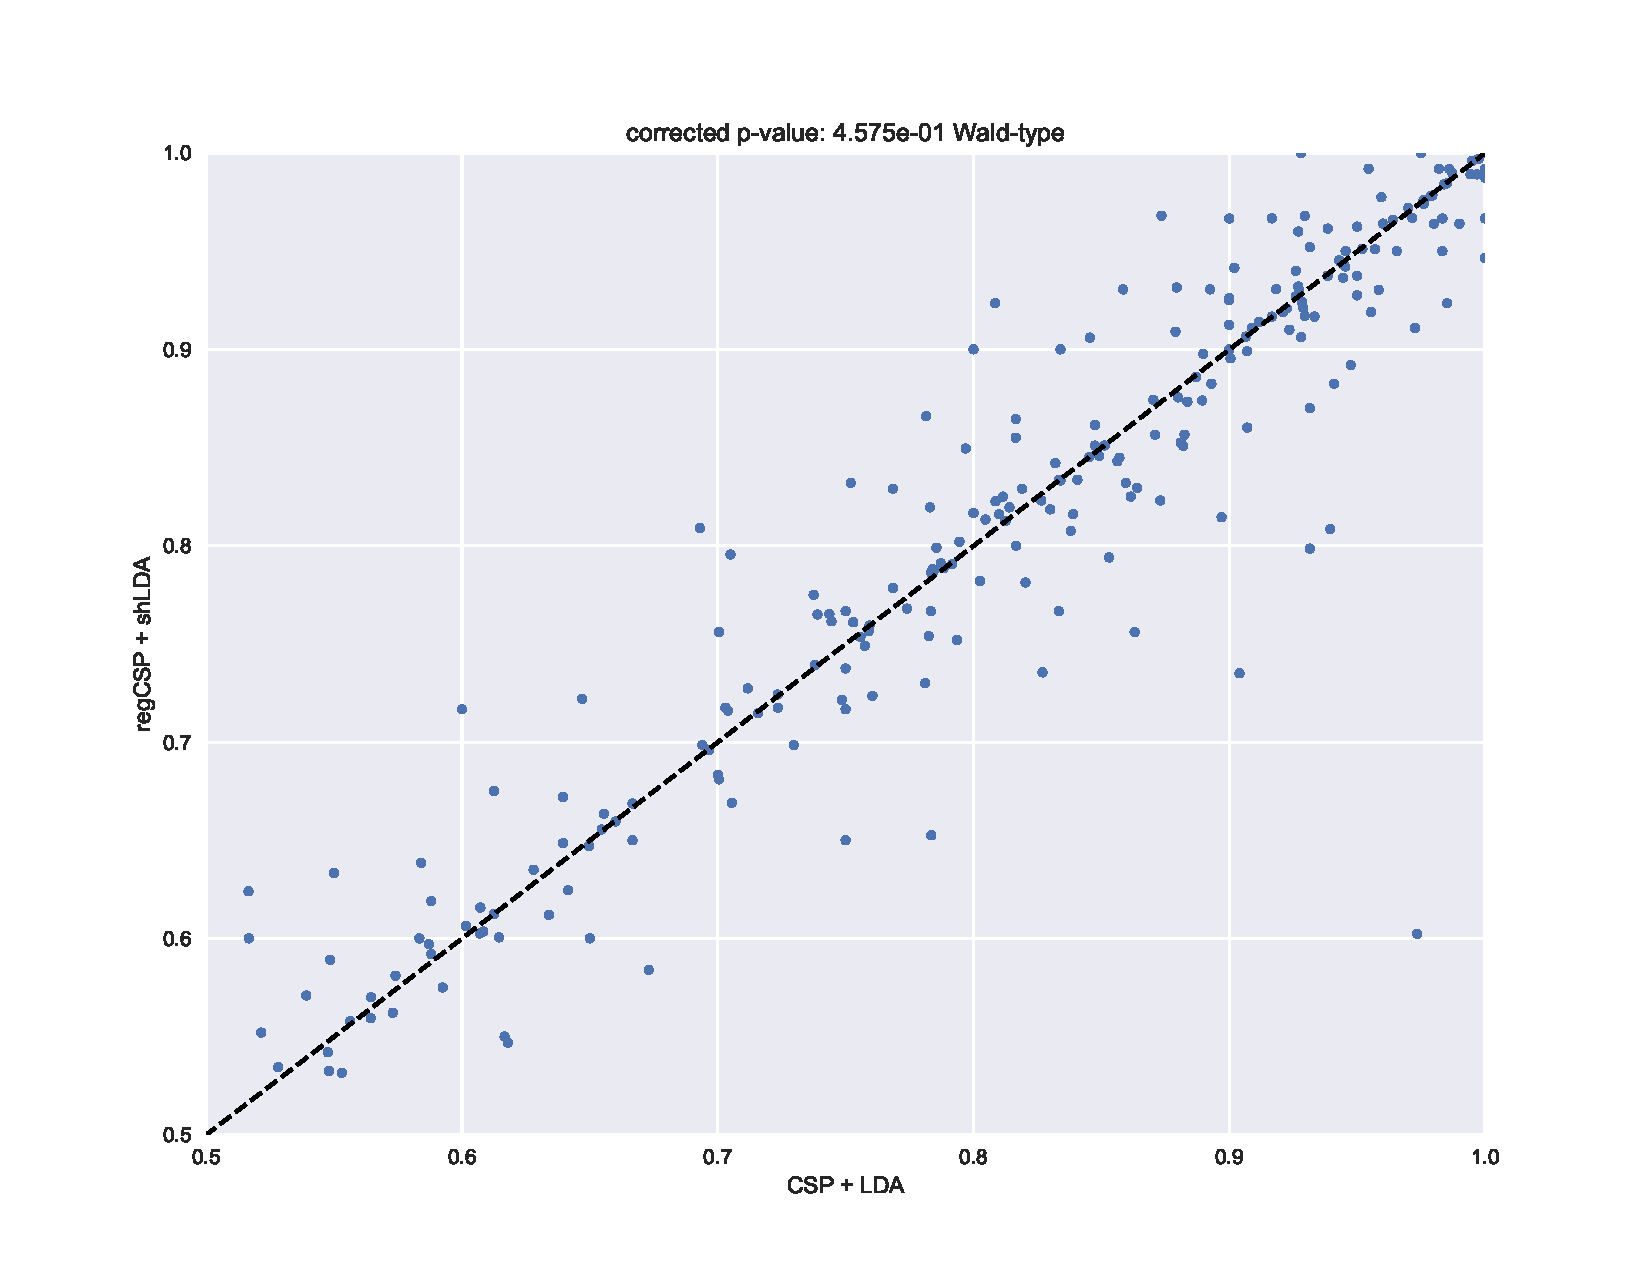
\includegraphics[width=\textwidth]{Figures/CSP1.pdf}
    \end{subfigure}%
    \begin{subfigure}{0.475\textwidth}
        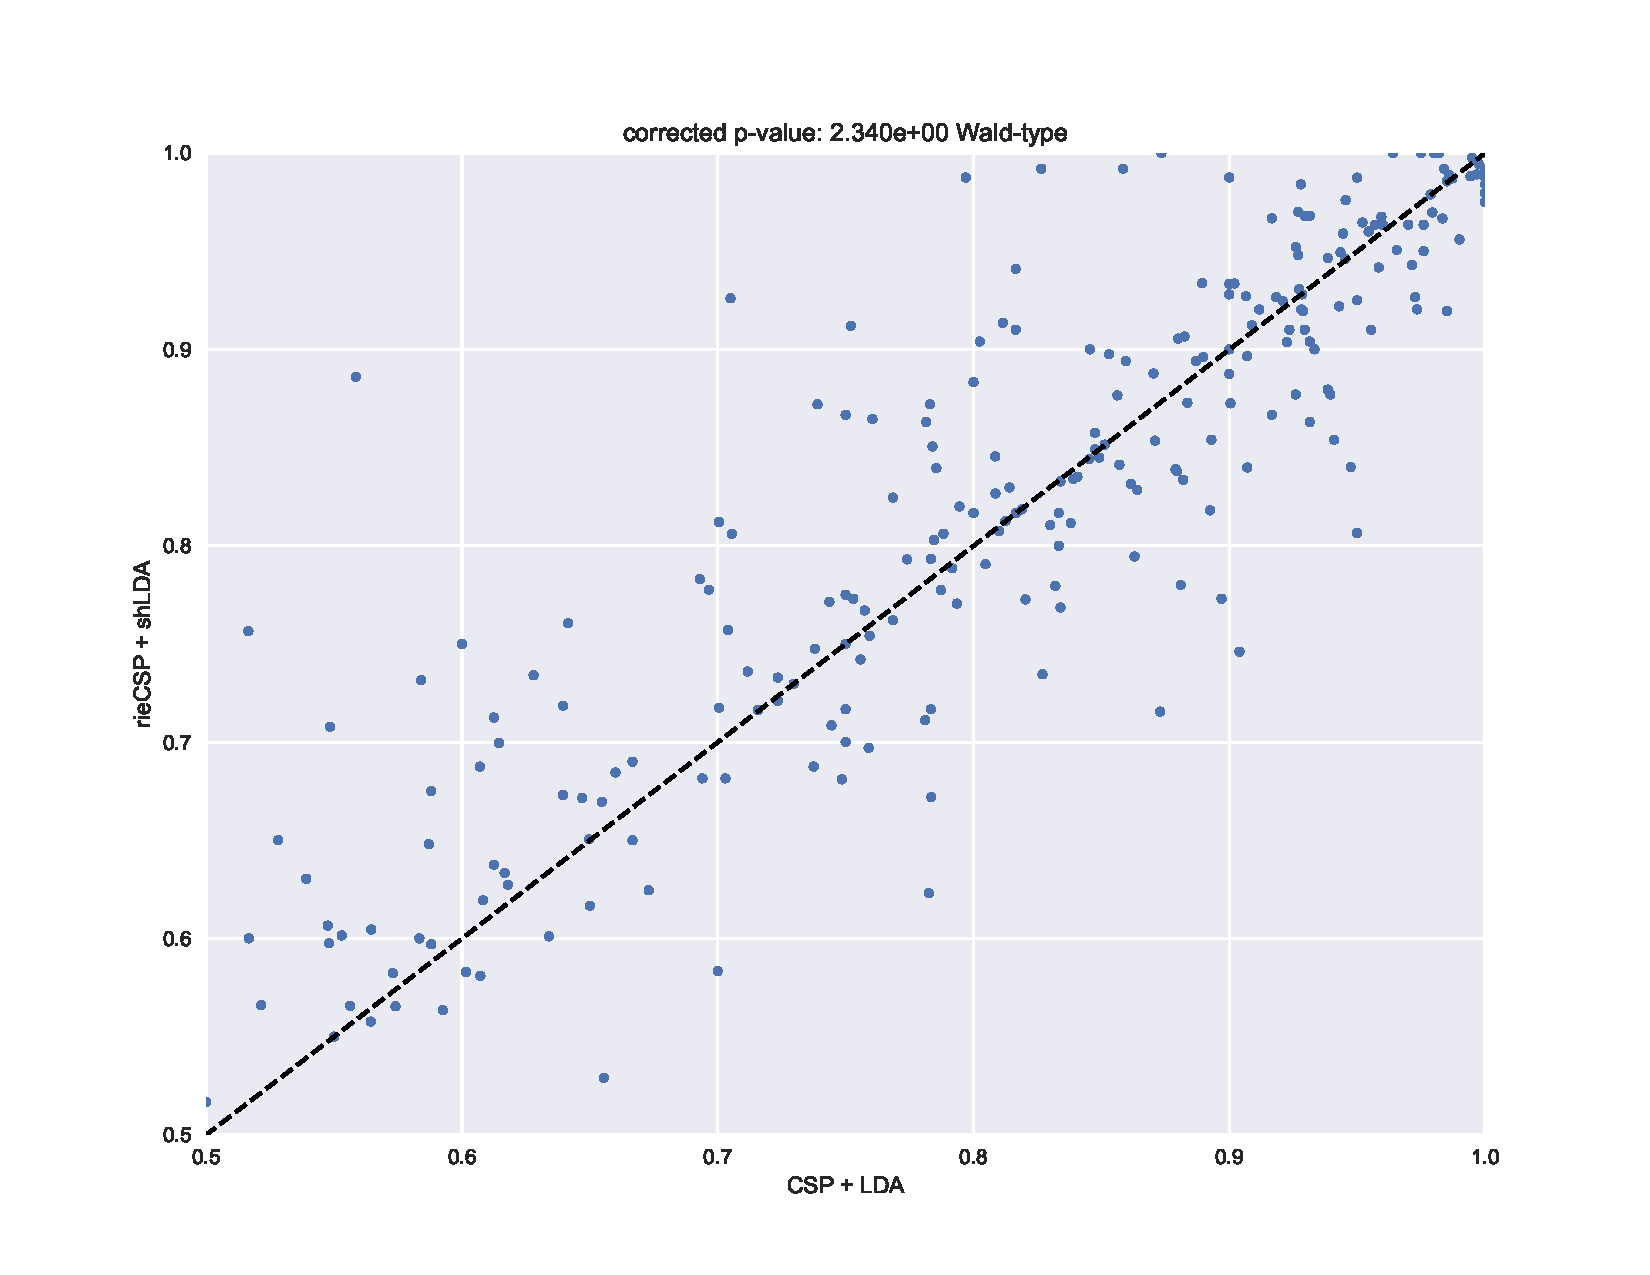
\includegraphics[width=\textwidth]{Figures/CSP2.pdf}
    \end{subfigure}
    \begin{subfigure}{0.475\textwidth}
        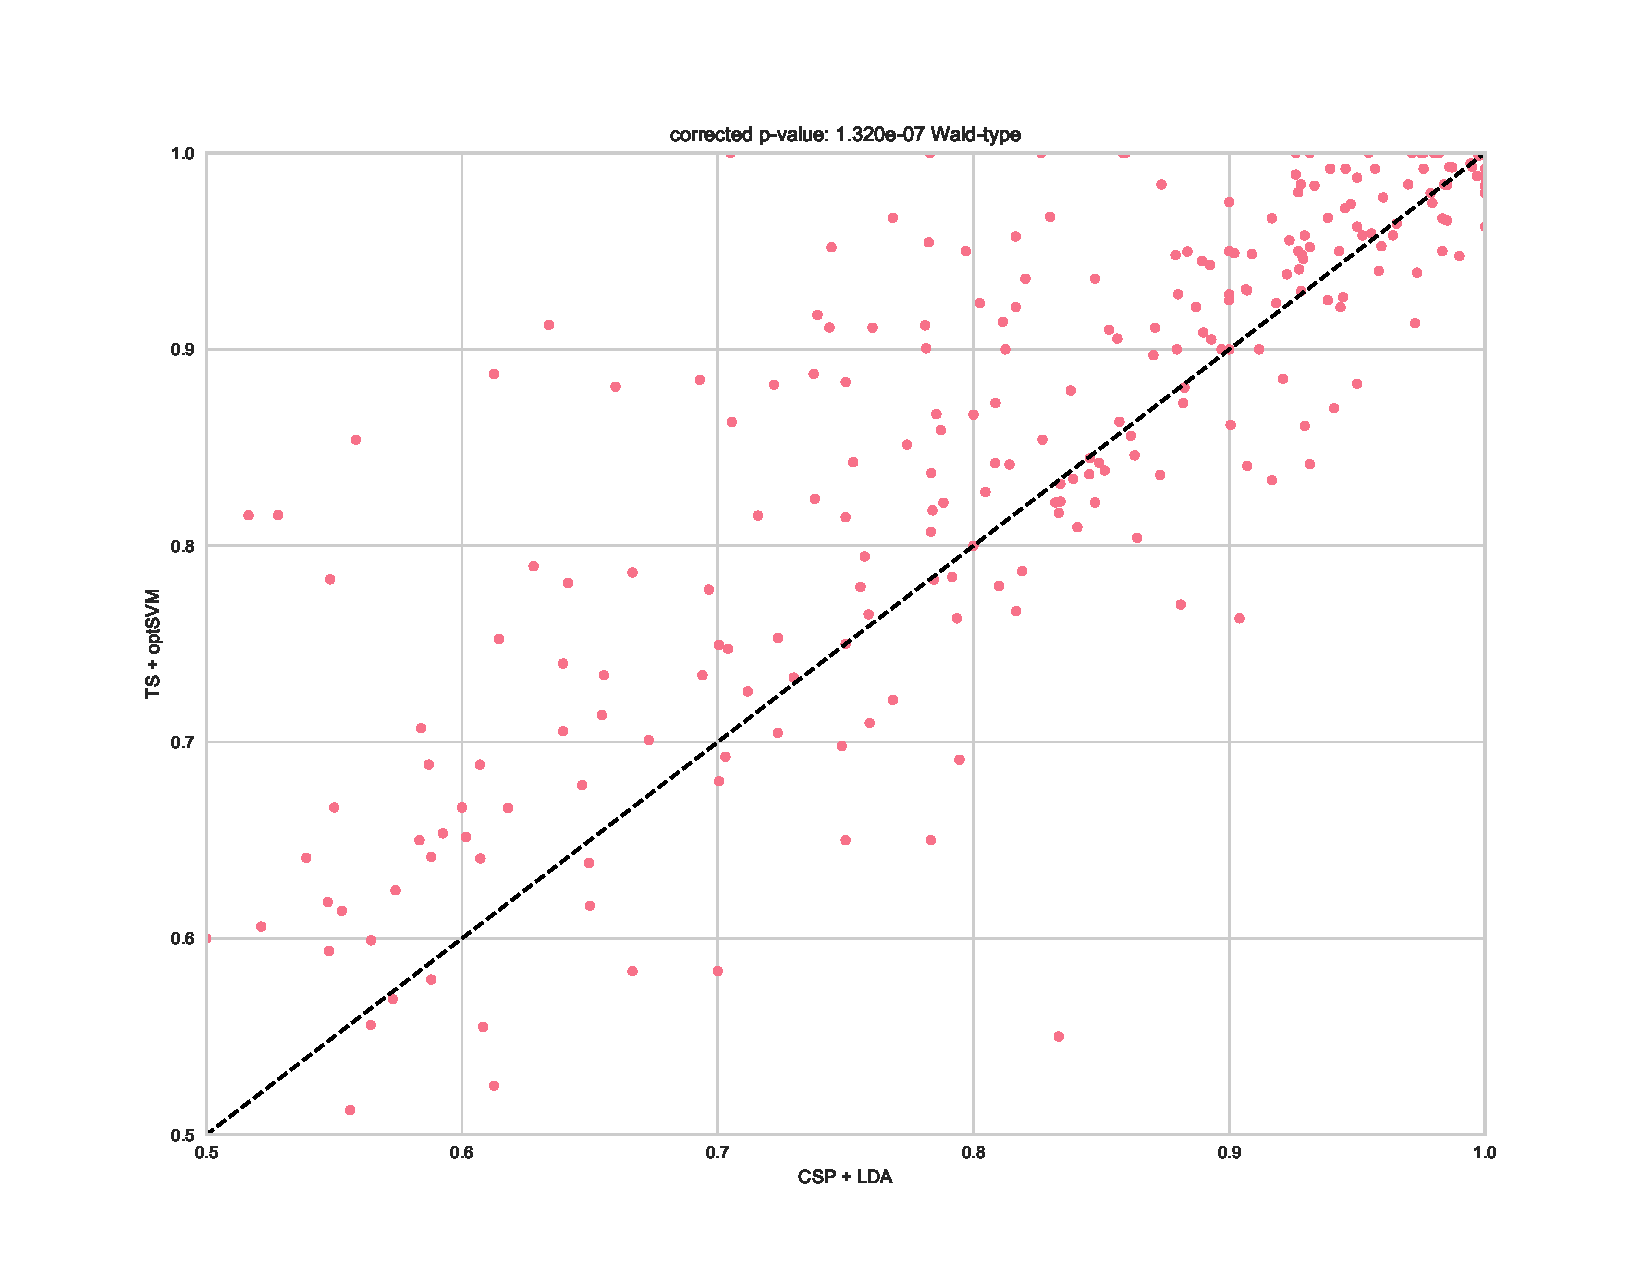
\includegraphics[width=\textwidth]{Figures/CSP3.pdf}
    \end{subfigure}
    \begin{subfigure}{0.475\textwidth}
        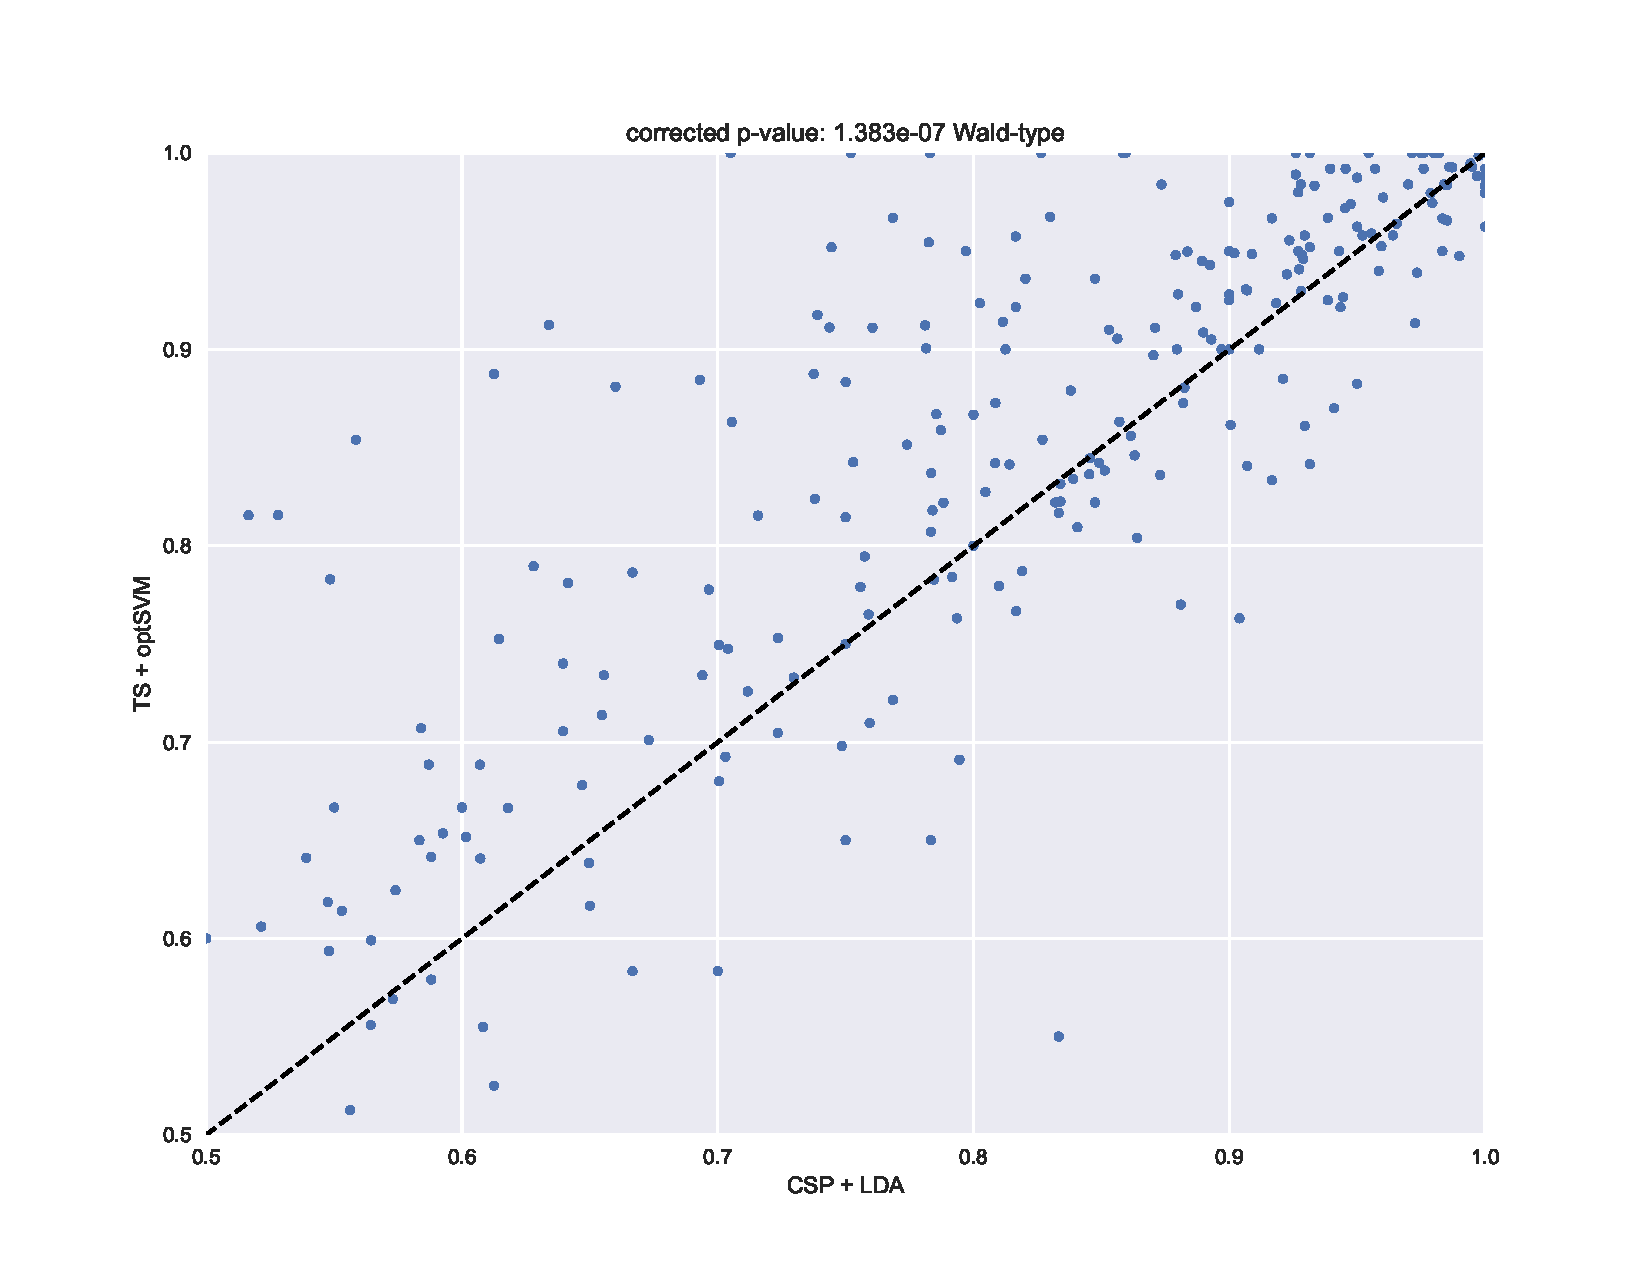
\includegraphics[width=\textwidth]{Figures/CSP4.pdf}
    \end{subfigure}
    \caption{Paired pots of CSP versus the two regularized methods, FBCSP, 
      and the tangent space SVM. Interestingly, across datasets
      neither of the regularization methods does significantly better
      in within-session classification. However, the tangent space
      method does reliably out-perform it}
    \label{fig:csp}
\end{figure*}
\begin{figure*}
  \centering
  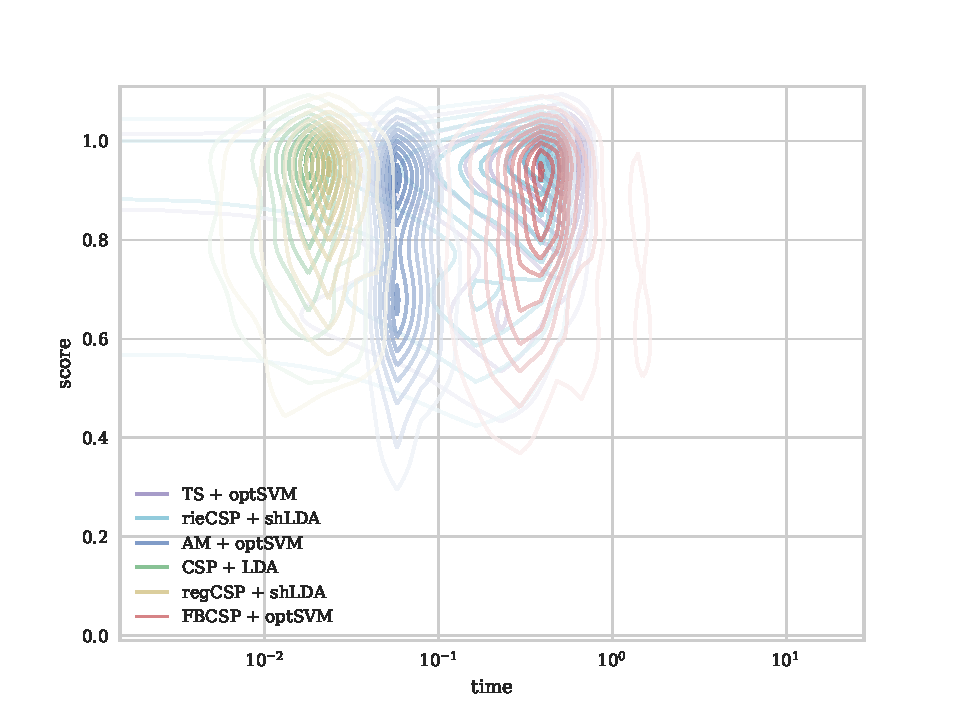
\includegraphics[width=\textwidth]{Figures/time_score.pdf}
  \caption{Plot of the distribution of score versus computation time over all
    datasets, for all pipelines. }
  \label{fig:time}
\end{figure*}

%%% Local Variables:
%%% mode: latex
%%% TeX-master: "main"
%%% End:
